%!TEX root = ../my_thesis.tex
\section{Opposite-side electron optimisation}
\label{app:oselectronappendix}

The correlation between the predicted mistag $\eta$ and the input features is shown in Figs.~\ref{fig:OSepartialdependenceRunI},~\ref{fig:OSepartialdependenceRunIIB2CC} and~\ref{fig:OSepartialdependenceRunIIB2OC}  for the Run 1 new, Run 2 B2CC and Run 2 B2OC implementations of the \OSe~tagger, respectively. This correlation, known as \emph{partial dependence}, allows to check the impact of each feature on the classifier, in addition to the F-score (Sec.~\ref{sec:tagging:OSeBDT}).

\begin{figure}[t]
        \centering
        \includegraphics[width=0.8\textwidth]{04FlavourTagging/figs/OSelectronOpt/2017-12-12-vibattis-OSElectron-bdt-calibration-sWeights_Run1/PartialDependence_RunIcuts.pdf}
        \vspace{-2mm}
        \caption{Partial dependence of the predicted mistag $\eta$ (\OSe~Run 1 tagger) for each feature used as BDT input, marginalised over any other feature. The blue two-dimensional distributions represent the \emph{sWeighted} data, whereas the red line shows the average $\eta$ for each feature bin.}
         \label{fig:OSepartialdependenceRunI}
\end{figure}

\begin{figure}[t]
        \centering
        \includegraphics[width=\textwidth]{04FlavourTagging/figs/OSelectronOpt/2017-12-12-vibattis-OSElectron-bdt-calibration-sWeights_Run2/PartialDependence_RunIIcuts.pdf}
        \vspace{-2mm}
        \caption{Partial dependence of the predicted mistag $\eta$ (\OSe~Run 2 B2CC tagger) for each feature used as BDT input, marginalised over any other feature. The blue two-dimensional distributions represent the \emph{sWeighted} data, whereas the red line shows the average $\eta$ for each feature bin.}
        \label{fig:OSepartialdependenceRunIIB2CC}
\end{figure}

\begin{figure}[t]
        \centering
        \includegraphics[width=\textwidth]{04FlavourTagging/figs/OSelectronOpt/2018-04-07-vibattis-OSElectron-bdt-calibration-sWeights_Run2_Bu2D0pi/PartialDependence_RunIIcuts.pdf}
        \vspace{-2mm}
        \caption{Partial dependence of the predicted mistag $\eta$ (\OSe~Run 2 B2OC tagger) for each feature used as BDT input, marginalised over any other feature. The blue two-dimensional distributions represent the \emph{sWeighted} data, whereas the red line shows the average $\eta$ for each feature bin.}
        \label{fig:OSepartialdependenceRunIIB2OC}
\end{figure}

An important step in the BDT development is the hyperparameter tuning. In particular, the maximum depth (md) of each tree of the ensemble and the number of trees (nt) are optimised. In order to do so, a cross-validation+bootstrapping procedure is followed:
\begin{itemize}[noitemsep,topsep=0pt]
  \item For a given set of maximum depth and number of trees values, the training set is bootstrapped 10 times. Each bootstrapped sample is then divided in three exclusive subsamples.
  \item The first subsample is used to train a BDT. The BDT is then transformed into a mistag probability, and a calibration is performed on the second subsample (a simple second order logistic function is used). Finally, the calibration is applied on the third sample, where the per-event tagging power is computed. The ROC AUC is also obtained as additional performance metric.
  \item The above procedure is repeated by permutating the 3 samples. This means that, in total, there are $3\times10=30$ approximately independent estimations of the BDT performance for each set of hyperparameters. The average tagging power and ROC AUC values are finally computed over the 30 estimations, together with the standard error on the mean.   
\end{itemize}
The result for the Run 1 new \OSe~algorithm is shown in Fig.~\ref{fig:OSecrossvalidationRunI}. The performance is weakly dependent on the hyperparameters. For this reason, the maximum depth and the number of trees are fixed to 3 and 300 respectively, in order to reduce complexity. A similar result is observed for the Run 2 B2OC and Run 2 B2CC \OSe~algorithms.

\begin{figure}[t]
  \centering
        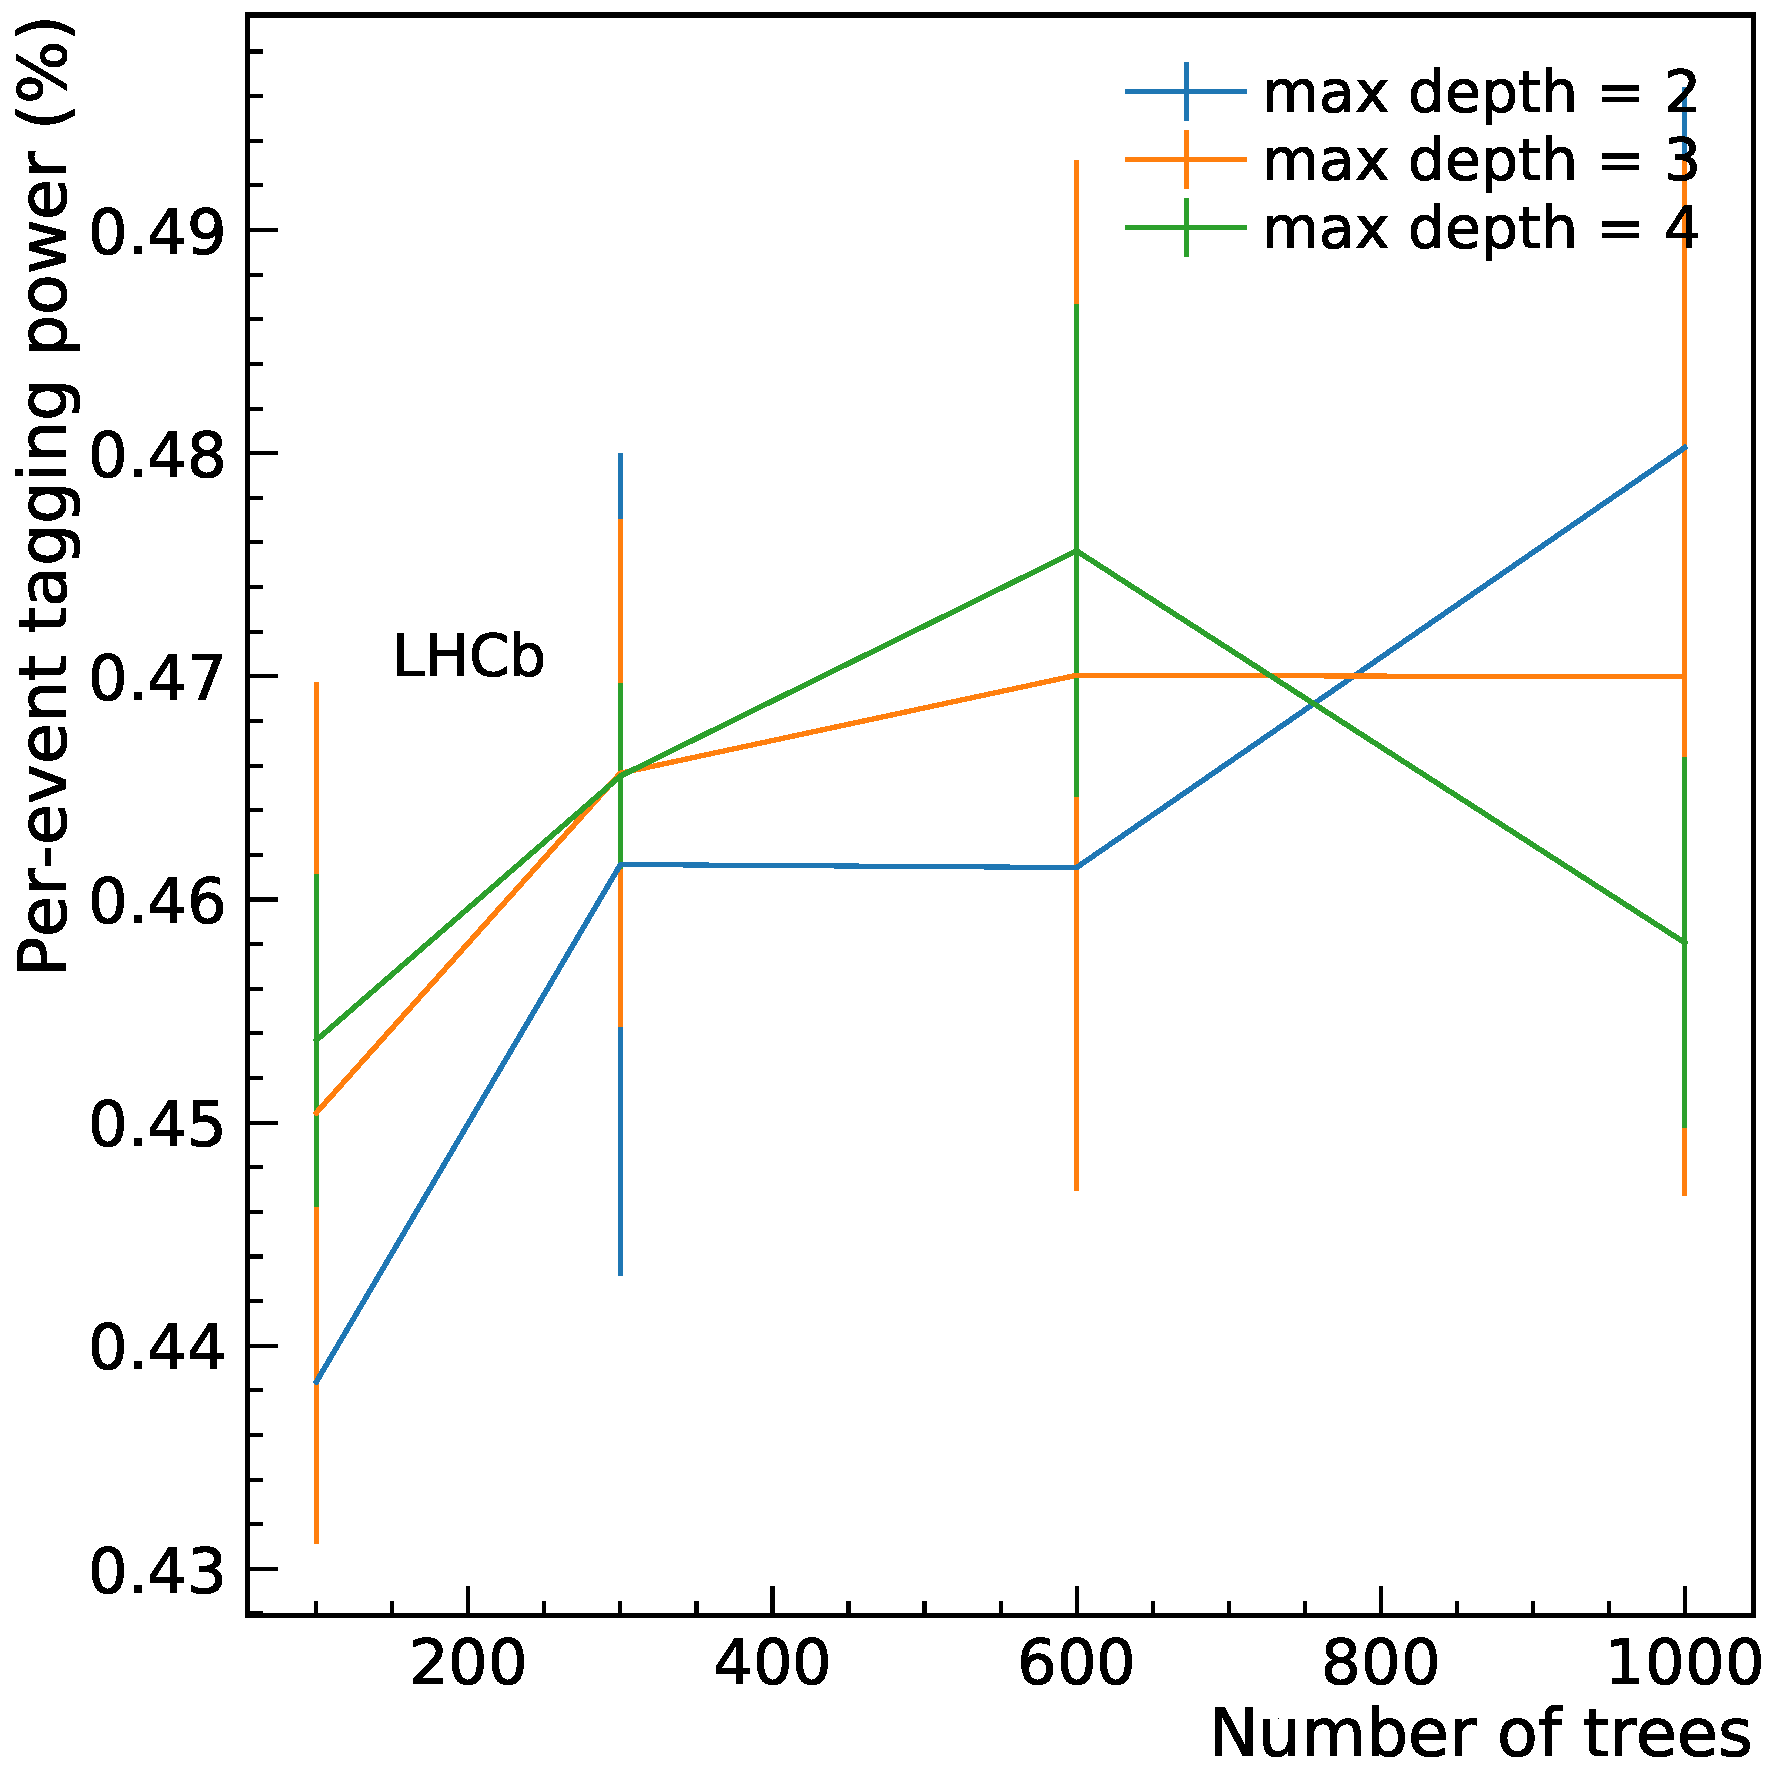
\includegraphics[width=0.4\textwidth]{04FlavourTagging/figs/OSelectronOpt/2018-01-09-vibattis-OSElectron-bdt-crossvalidation-sWeights_Run1/crossval_tp.pdf}
        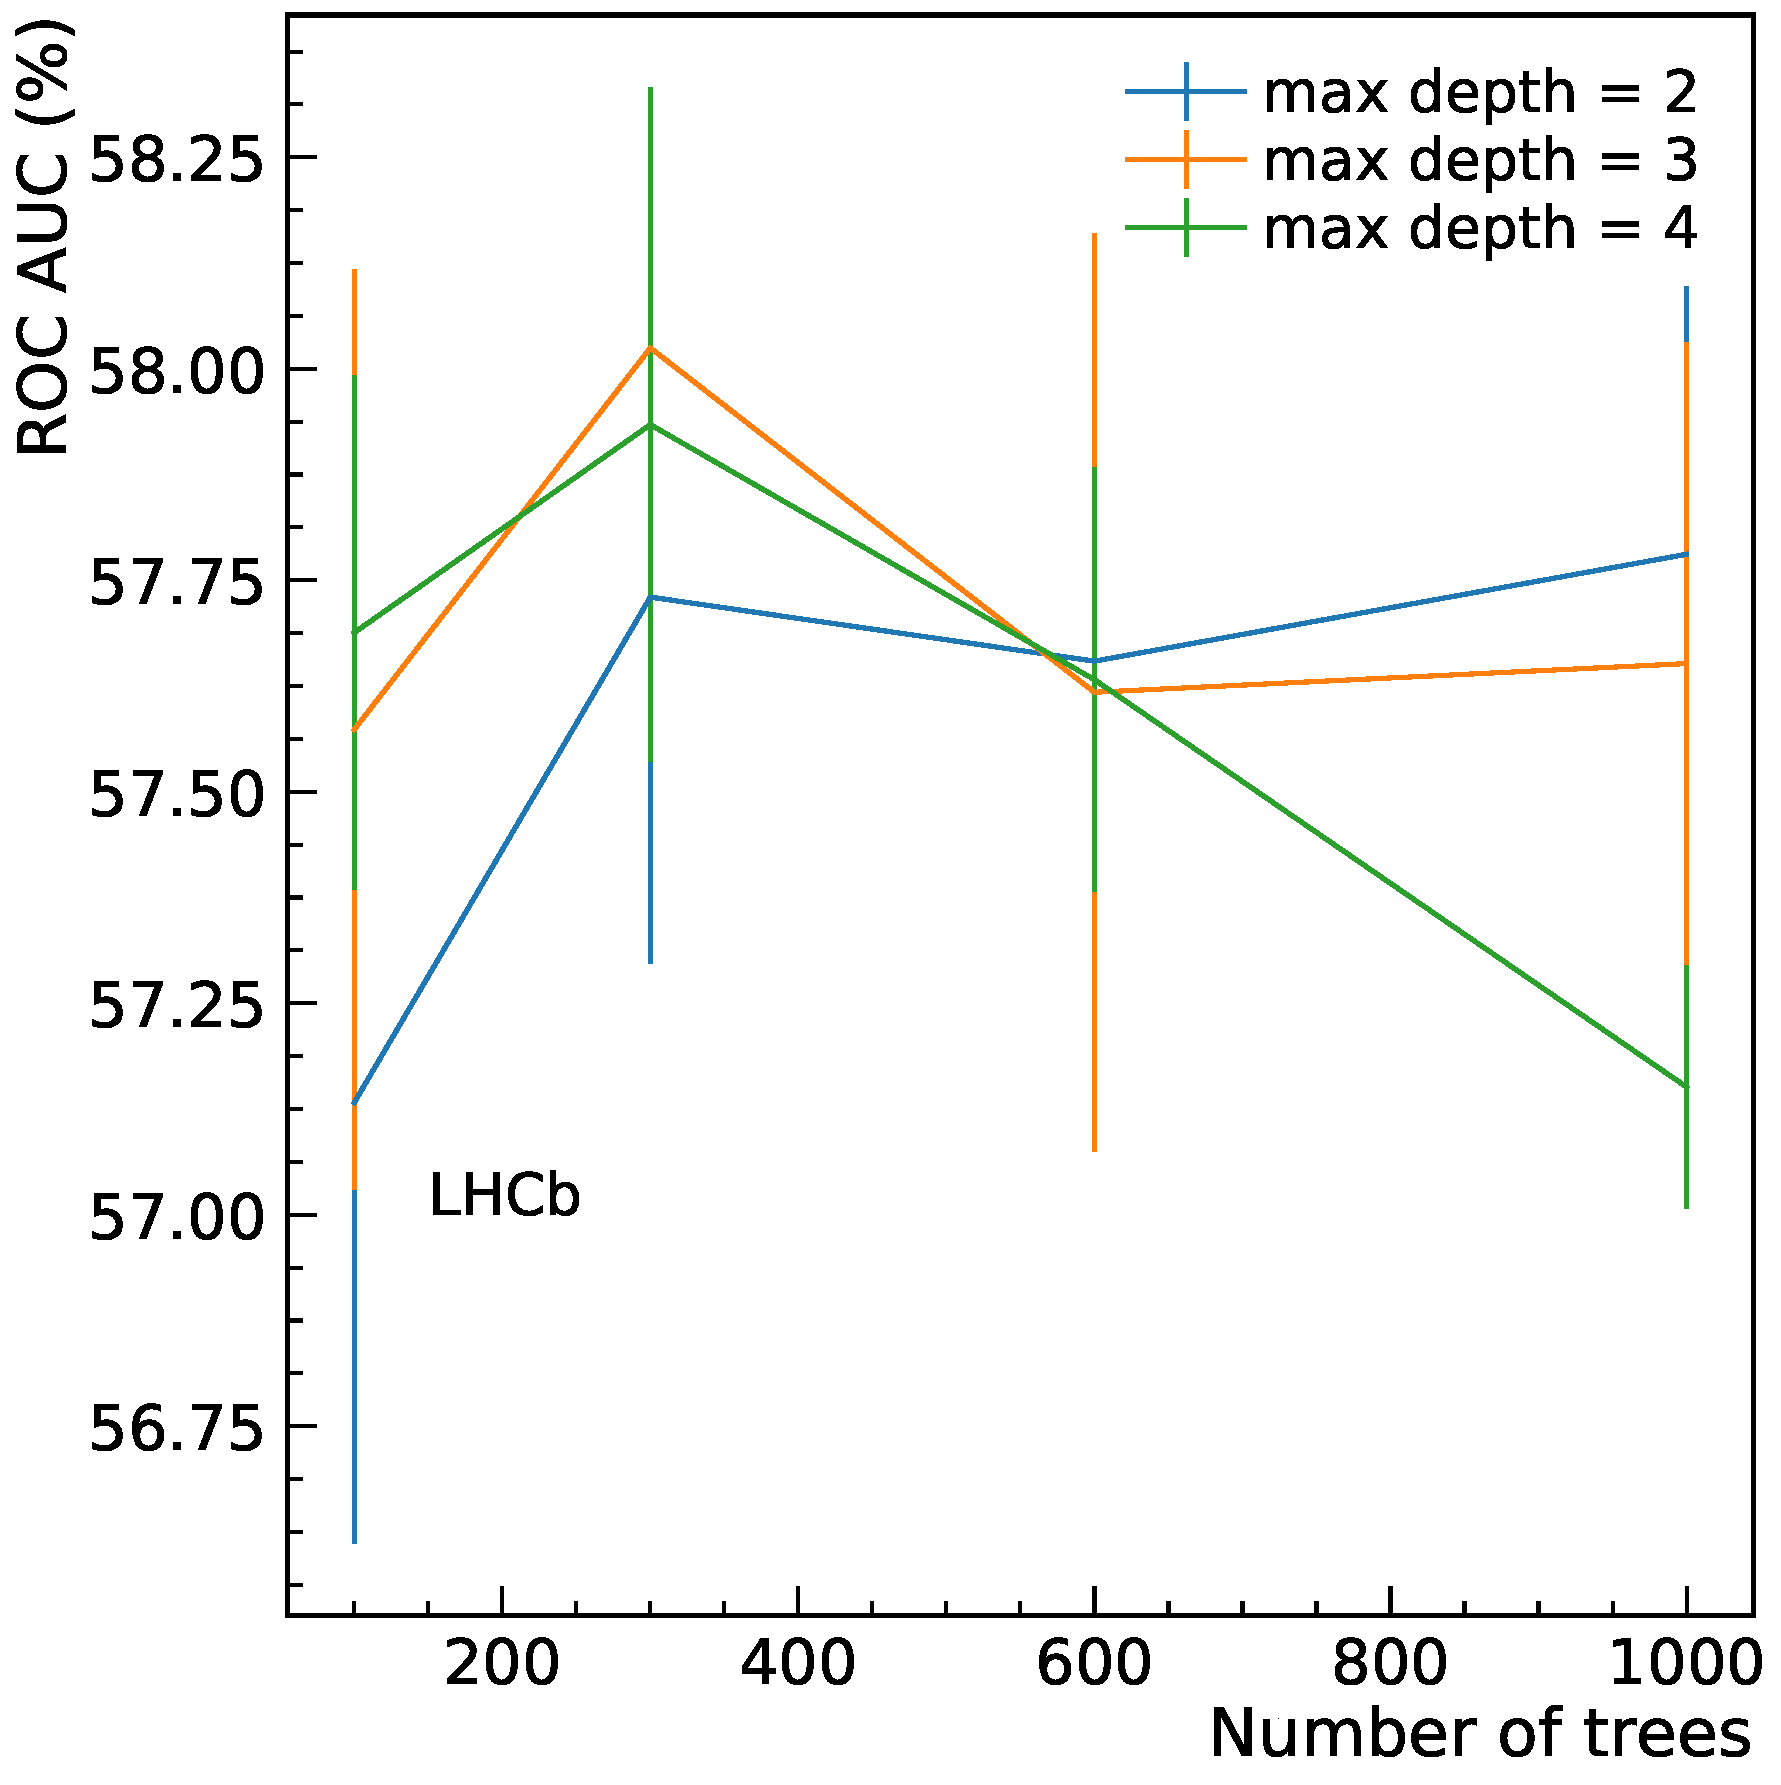
\includegraphics[width=0.4\textwidth]{04FlavourTagging/figs/OSelectronOpt/2018-01-09-vibattis-OSElectron-bdt-crossvalidation-sWeights_Run1/crossval_roc_auc.pdf} \\
        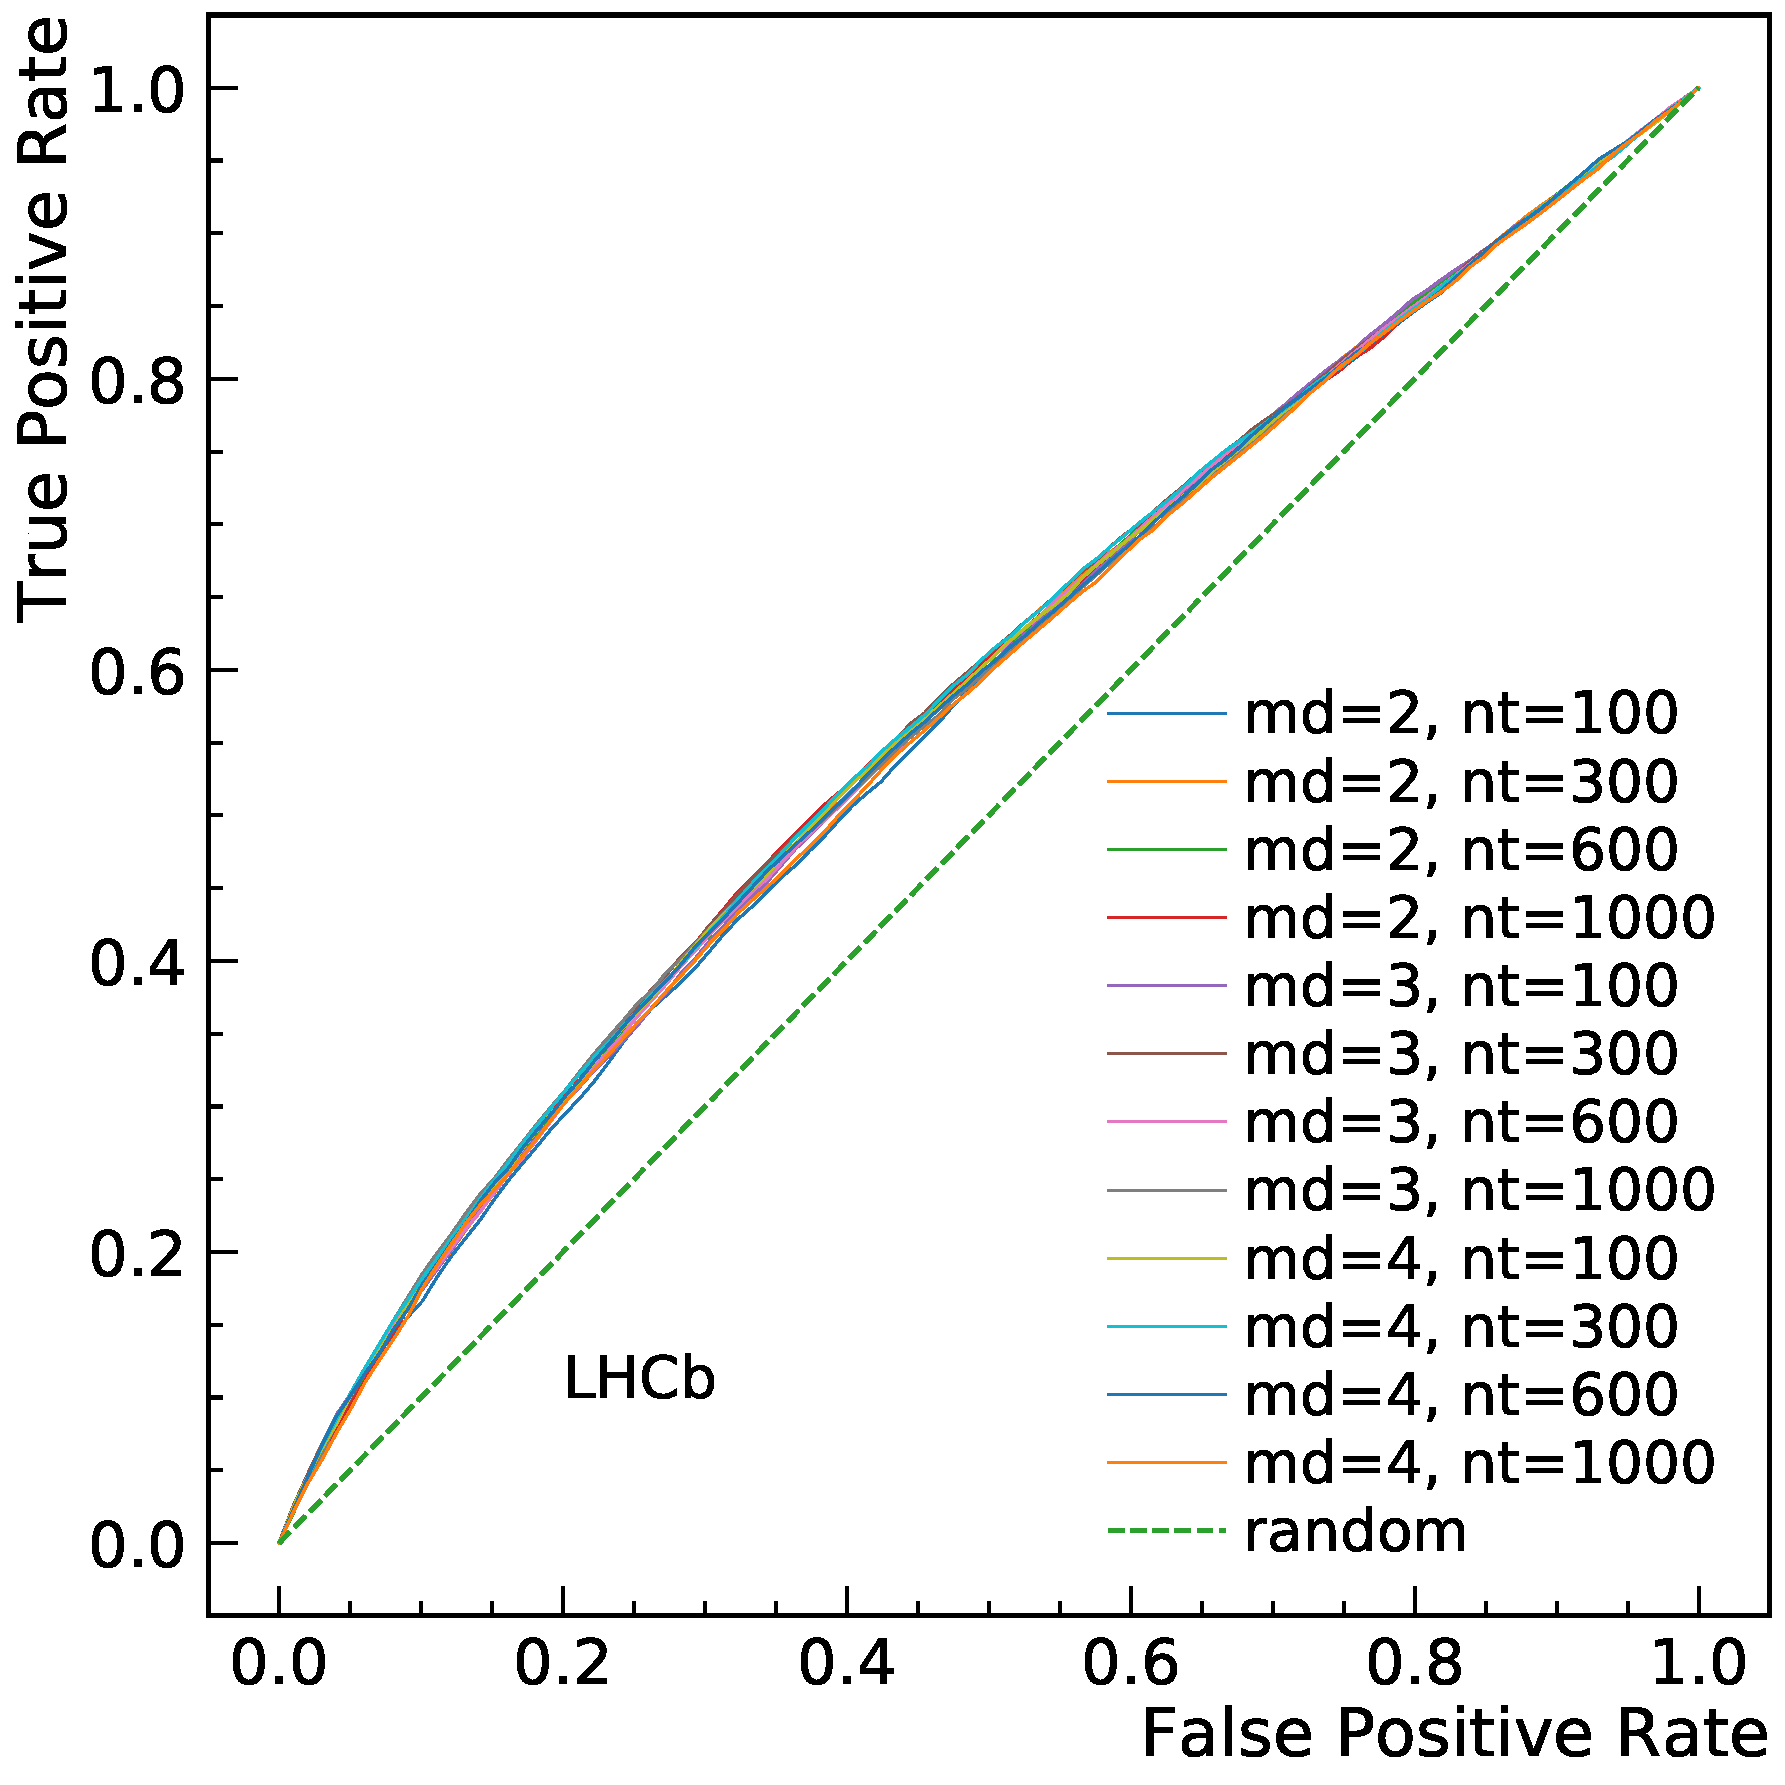
\includegraphics[width=0.4\textwidth]{04FlavourTagging/figs/OSelectronOpt/2018-01-09-vibattis-OSElectron-bdt-crossvalidation-sWeights_Run1/roc_curve.pdf} \\
        \vspace{-2mm}
        \caption{Tagging power (top left), ROC AUC (top right), and ROC curve (bottom) for each set of hyperparameters considered
          for the tuning of the BDT classifier used for the mistag estimation by the Run 1 new version of the \OSe~tagger (cross-validation).}
        \label{fig:OSecrossvalidationRunI}
\end{figure}
